\chapter{Klasser}
Formålet med dette afsnit er at gøre rede for hvorledes forskellige typer output led der kan bruges i en hi-fi forstærker og hvad fordele og ulemper der er ved dem. Denne redegørelse skal udmunde i en afgørelse om hvilken type output led der vælges til dette projekt.

\section{Klasse A}

\begin{figure}[h]
\centering
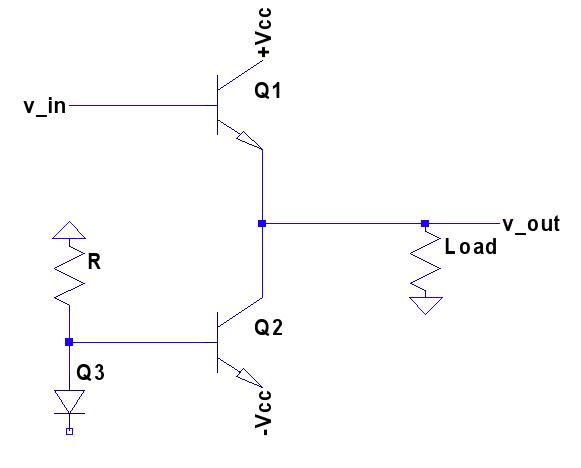
\includegraphics[scale=.6]{klasser/classa.png}
\caption{Klasse A forstærker kredsløb.}
\label{fig:classa}
\end{figure}


\section{Klasse B}
En klasse B forstærker er opbygget af to transistorer, en NPN (Q1) og en PNP (Q2), som vist på figur \ref{fig:classb}. Når input spændingen overstiger ca. 0,5 V vil Q1 begynde at lede strøm til loadmodstanden mens Q2 er lukket. Kommer input spændingen under -0,5 V vil Q2 lede, men da Q2 er en PNP vil den trække strøm mod -Vcc hvormed der trækkes strøm fra loadmodstanden. Når Q2 leder er Q1 lukket. 
Der afsættes ikke nær så meget effekt i en klasse B forstærker når input spændingen er 0 V, som i en klasse A. Dette skyldes at klasse B har et dødområde, grundet transistorerne saturation-spænding. Dødområdet er, i ovenstående eksempel, på +-0,5 V. 

\begin{figure}[h]
\centering
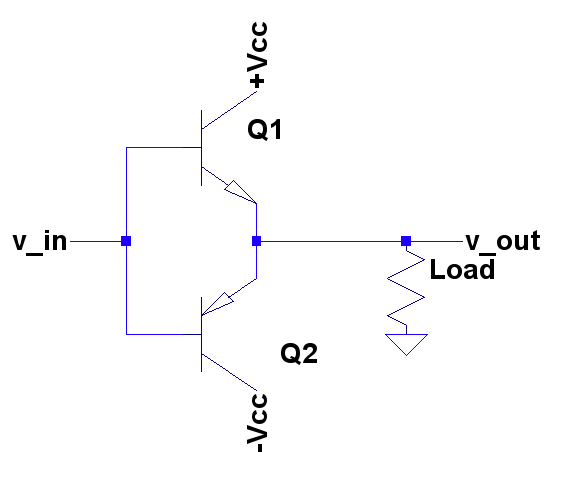
\includegraphics[scale=.6]{klasser/classb.png}
\caption{Klasse B forstærker kredsløb.}
\label{fig:classb}
\end{figure}

\section{Klasse AB}
\begin{figure}[h]
\centering
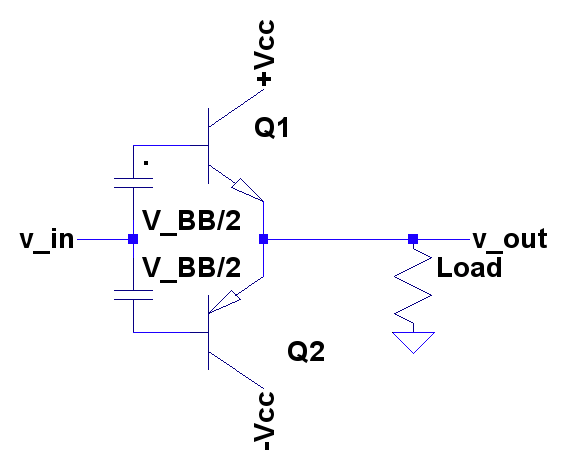
\includegraphics[scale=.6]{klasser/classab.png}
\caption{Klasse AB forstærker kredsløb.}
\label{fig:classab}
\end{figure}